\appendix
\chapter{Raw Results}
\label{cha:appendix}

\chapter{Simulation Setup}
%Use this chapter for simulation setup information

\section{Ferrotec 9500-035-085 B CFD Modelling}
\label{cha:app_TEC_CFD}

\section{CFD Simulation Convergence Data}
\label{cha:CFDconverg}
%NEED data of CFD convergence here for initial sim

Figure \ref{fig:2tecconv} shows the convergence plot for the refined, 2 TEC design simulation.

\begin{figure}[!htb]
	\centering
	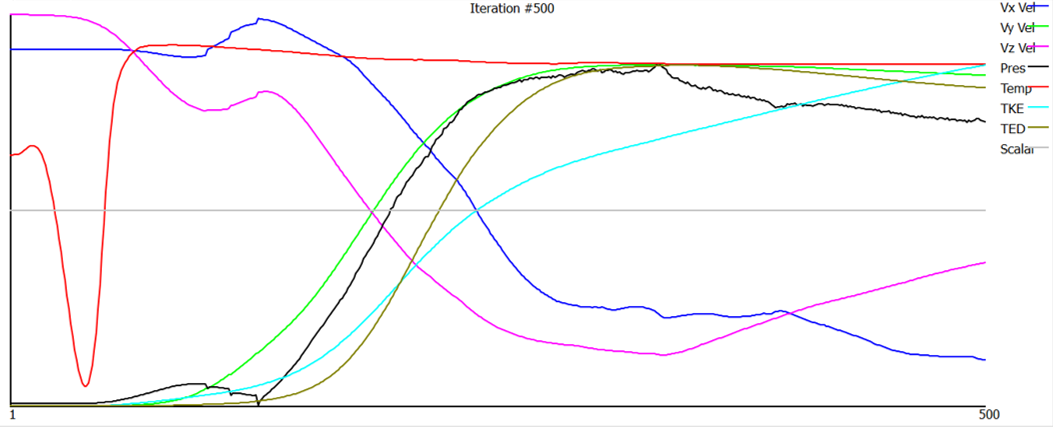
\includegraphics[width = \textwidth]{2tecconv.png}
	\caption[Convergence Plot for Refined Design CFD.]{Convergence Plot for Refined Design CFD.}
	\label{fig:2tecconv}
\end{figure}ˆ 
\FloatBarrier







% Here's an example of how to rotate the page so you can fit large tables
%
%\begin{landscape}
%\begin{table}[h!] 
%\begin{center} \begin{tabular}{rrrrr}\hline 
%Q & W & E & R & T \\ \hline 
%AAAAAAAAAAAAAAA & 111111111111111 & 222222222222222 & 333333333333333 & 444444444444444 \\ 
%BBBBBBBBBBBBBBB & 555555555555555 & 666666666666666 & 777777777777777 & 888888888888888 \\ \hline 
%\end{tabular} \end{center}
%\caption[Short Name]{Longer name} 
%\label{tab:appendix_tablename} 
%\end{table} 
%\end{landscape}